\documentclass[10pt, portrait,letterpaper]{article}

\usepackage[utf8]{inputenc} 
\usepackage[russian]{babel} 
\usepackage{amsmath}
\usepackage{amssymb}
\usepackage{siunitx} % for \num
\usepackage{hyperref} 
\usepackage[dvips]{graphicx} % Картинки у Михаила Иванова
%\usepackage[pdflatex]{graphicx} % Картинки у Егора Горбачёва
\usepackage[a4paper, margin=.5in, top=1in]{geometry}
\usepackage{fancyhdr}
\usepackage{lastpage}
\usepackage{cmap}
\usepackage{mleftright}
\pagestyle{fancy}
\def\le{\leqslant}
\def\leq{\leqslant}
\def\ge{\geqslant}
\def\geq{\geqslant}
\def\xor{\mathbin{\mathrm{XOR}}}
\renewcommand{\headrulewidth}{1pt}
\lhead{SPbSU: Urgant Team (Grigoryev, Ivanov, Karpovich) }\chead{}\rhead{Page \thepage\ of \pageref{LastPage}}
\lfoot{}\cfoot{}\rfoot{}
\title{NERC 2022}
\date{29 октября 2022}
\author{SPbSU: Urgant Team (Grigoryev, Ivanov, Karpovich) }

\begin{document}
%\section{$\mathbb{R}$}
\tableofcontents
%\maketitle
%\addtocounter{page}{1}
%\addtocounter{chapter}{1}
\onecolumn

%add: halfplanes

\section{Общее}

\subsection{Пробный тур}

1. Первым делом почекать, считаются ли WA и CE за попытки. Можно ли засылать в уже сданную задачу?

2. Пописать код и посдавать каждому члену команды.

3. Сравнить скорости компа и тестирующей системы на Флойде ($n \sim 1050$).

4. Запустить все IDE, проверить, что все настройки работают, проверить, что работает C++11.

5. Проверить, есть ли \texttt{int128}.

6. Проверить работу прагм в тестирующей системе.

7. Почекать максимальный размер отправляемого кода.

8. Проверить рабочесть стресса.

\subsection{Чеклист при отправке}

1. Протестить на всех тестах из примера и других рандомных тестах.

2. Протестить все крайние случаи.

3. Убрать дебаг вывод.

4. Точно убедиться в правильности ответа и формата вывода.

5. Перечитать формат ввода/вывода.

6. Проверить, все ли хорошо с мультитестом.


\subsection{Факты из жизни IMO KINGS}
\begin{itemize}
    \item 1 января 2000 года~-- суббота, 1 января 1900 года~-- понедельник.
    \item Високосные года: если $400\mid a$, либо если $4\mid a$, но не $100\mid a$.
    \item $\mathtt{INT\_MIN} = -2\,147\,483\,648$, $\mathtt{INT\_MAX} = 2\,147\,483\,647$, $\mathtt{UINT\_MAX} = 4\,294\,967\,295$, 
    \item $\mathtt{SHRT\_MIN} = -32\,768$, $\mathtt{SHRT\_MAX} = 32\,767$, $\mathtt{LLONG\_MIN} = -9\,223\,372\,036\,854\,775\,808$,
    \item $\mathtt{LLONG\_MAX} = 9\,223\,372\,036\,854\,775\,807$, $\mathtt{ULLONG\_MAX} = 18\,446\,744\,073\,709\,551\,615$.
\end{itemize}

{\scriptsize
\begin{center}
\begin{tabular}{|c|c|c|c|c|c|c|c|c|c|c|c|c|c|c|c|c|c|}
		\hline
	$10^{1}$ & $10^{2}$ & $10^{3}$ & $10^{4}$ & $10^{5}$ & $10^{6}$ & $10^{7}$ & $10^{8}$ & $10^{9}$ & $10^{10}$ & $10^{11}$ & $10^{12}$ & $10^{13}$ & $10^{14}$ & $10^{15}$ & $10^{16}$ & $10^{17}$ & $10^{18}$ \\
		\hline
	 & $-47$ & $-63$ & $-113$ & $-123$ & $-137$ & $-111$ & $-213$ & $-267$ & $-231$ & $-231$ & $-233$ & $-447$ & $-203$ & $-429$ & $-369$ & $-413$ & $-369$ \\
		\hline
	 & $-41$ & $-59$ & $-99$ & $-119$ & $-117$ & $-99$ & $-179$ & $-261$ & $-219$ & $-179$ & $-153$ & $-411$ & $-179$ & $-423$ & $-359$ & $-273$ & $-363$ \\
		\hline
	 & $-39$ & $-53$ & $-93$ & $-99$ & $-93$ & $-93$ & $-173$ & $-249$ & $-213$ & $-171$ & $-143$ & $-357$ & $-171$ & $-357$ & $-357$ & $-261$ & $-291$ \\
		\hline
	 & $-33$ & $-47$ & $-77$ & $-93$ & $-83$ & $-71$ & $-161$ & $-243$ & $-183$ & $-167$ & $-137$ & $-341$ & $-147$ & $-341$ & $-329$ & $-239$ & $-263$ \\
		\hline
	 & $-29$ & $-33$ & $-71$ & $-77$ & $-69$ & $-69$ & $-153$ & $-239$ & $-167$ & $-149$ & $-123$ & $-299$ & $-77$ & $-191$ & $-191$ & $-177$ & $-251$ \\
		\hline
	 & $-27$ & $-29$ & $-69$ & $-71$ & $-47$ & $-63$ & $-69$ & $-203$ & $-149$ & $-129$ & $-101$ & $-267$ & $-71$ & $-173$ & $-183$ & $-81$ & $-171$ \\
		\hline
	$-8$ & $-21$ & $-23$ & $-59$ & $-39$ & $-41$ & $-57$ & $-59$ & $-117$ & $-119$ & $-93$ & $-63$ & $-237$ & $-69$ & $-123$ & $-149$ & $-57$ & $-137$ \\
		\hline
	$-7$ & $-17$ & $-17$ & $-51$ & $-29$ & $-39$ & $-29$ & $-41$ & $-107$ & $-71$ & $-57$ & $-41$ & $-201$ & $-41$ & $-117$ & $-113$ & $-39$ & $-123$ \\
		\hline
	$-5$ & $-11$ & $-9$ & $-33$ & $-11$ & $-21$ & $-27$ & $-29$ & $-71$ & $-57$ & $-53$ & $-39$ & $-137$ & $-29$ & $-53$ & $-83$ & $-23$ & $-33$ \\
		\hline
	$-3$ & $-3$ & $-3$ & $-27$ & $-9$ & $-17$ & $-9$ & $-11$ & $-63$ & $-33$ & $-23$ & $-11$ & $-29$ & $-27$ & $-11$ & $-63$ & $-3$ & $-11$ \\
		\hline\hline
	$+1$ & $+1$ & $+9$ & $+7$ & $+3$ & $+3$ & $+19$ & $+7$ & $+7$ & $+19$ & $+3$ & $+39$ & $+37$ & $+31$ & $+37$ & $+61$ & $+3$ & $+3$ \\
		\hline
	$+3$ & $+3$ & $+13$ & $+9$ & $+19$ & $+33$ & $+79$ & $+37$ & $+9$ & $+33$ & $+19$ & $+61$ & $+51$ & $+67$ & $+91$ & $+69$ & $+13$ & $+9$ \\
		\hline
	$+7$ & $+7$ & $+19$ & $+37$ & $+43$ & $+37$ & $+103$ & $+39$ & $+21$ & $+61$ & $+57$ & $+63$ & $+99$ & $+97$ & $+159$ & $+79$ & $+19$ & $+31$ \\
		\hline
	$+9$ & $+9$ & $+21$ & $+39$ & $+49$ & $+39$ & $+121$ & $+49$ & $+33$ & $+69$ & $+63$ & $+91$ & $+129$ & $+99$ & $+187$ & $+99$ & $+21$ & $+79$ \\
		\hline
	$+13$ & $+13$ & $+31$ & $+61$ & $+57$ & $+81$ & $+139$ & $+73$ & $+87$ & $+97$ & $+69$ & $+121$ & $+183$ & $+133$ & $+223$ & $+453$ & $+49$ & $+177$ \\
		\hline
	$+19$ & $+27$ & $+33$ & $+67$ & $+69$ & $+99$ & $+141$ & $+81$ & $+93$ & $+103$ & $+73$ & $+163$ & $+259$ & $+139$ & $+241$ & $+481$ & $+81$ & $+183$ \\
		\hline
	$+21$ & $+31$ & $+39$ & $+69$ & $+103$ & $+117$ & $+169$ & $+123$ & $+97$ & $+121$ & $+91$ & $+169$ & $+267$ & $+169$ & $+249$ & $+597$ & $+99$ & $+201$ \\
		\hline
	$+27$ & $+37$ & $+49$ & $+79$ & $+109$ & $+121$ & $+189$ & $+127$ & $+103$ & $+141$ & $+103$ & $+177$ & $+273$ & $+183$ & $+259$ & $+613$ & $+141$ & $+283$ \\
		\hline
	$+31$ & $+39$ & $+51$ & $+91$ & $+129$ & $+133$ & $+223$ & $+193$ & $+123$ & $+147$ & $+129$ & $+189$ & $+279$ & $+261$ & $+273$ & $+639$ & $+181$ & $+381$ \\
		\hline
	$+33$ & $+49$ & $+61$ & $+93$ & $+151$ & $+151$ & $+229$ & $+213$ & $+181$ & $+207$ & $+171$ & $+193$ & $+283$ & $+357$ & $+279$ & $+669$ & $+337$ & $+387$ \\
		\hline
\end{tabular}
\end{center}
}

\subsection {Формулы}
\begin{itemize}
    \item  Расстояние между точками по сфере: $L = R \cdot \arccos(\cos\theta _1 \cdot \cos\theta _2 +\sin\theta _1 \cdot \sin\theta _2 \cdot \cos(\varphi _1 - \varphi _2))$, где $\theta$~-- широты (от $- \pi$ до $\pi$), $\varphi$~-- долготы (от $- \pi$ до $\pi$)
    \item Объем шарового сегмента: $V = \pi h^2(R - \frac{1}{3}h)$, где $h$~-- высота от вершины сектора до секущей плоскости
    \item Площадь поверхности шарового сегмента: $S = 2\pi Rh$, где $h$~-- высота
    \item $2^{23} \cdot 7 \cdot 17 + 1 = \num{998244353}$~-- простое, первообразный корень~-- 3
    \item Код Грея: $g_n = n \xor \frac{n}{2}$
    \item Числа Фибоначчи: $F_0 = 0, F_1 = 1, F_n = \dfrac{\left(\frac{1 + \sqrt{5}}{2}\right)^n - \left(\frac{1 - \sqrt{5}}{2}\right)^n}{\sqrt{5}}$
    \item Формула Кардано:
    \begin{itemize}
    	\item Переведём $ax^3+bx^2+cx+d=0$ при помощи $x=y-\frac b{3a}$ к виду $y^3+py+q=0$, где $p=\frac ca-\frac{b^2}{3a^2}=\frac{3ac-b^2}{3a^2}$, $q=\frac{2b^3}{27a^3}-\frac{bc}{3a^2}+\frac da=\frac{2b^3-9abc+27a^2d}{27a^3}$
    	\item $Q=\mleft(\frac p3\mright)^3+\mleft(\frac q2\mright)^2$, $\alpha=\sqrt[3]{-\frac q2+\sqrt Q}$, $\beta=\sqrt[3]{-\frac q2-\sqrt Q}$, $\Delta=-108Q$, $\alpha\beta=-\frac p3$
    	\item $y_1=\alpha+\beta$, $y_{2,3}=-\frac{\alpha+\beta}2\pm i\frac{\alpha-\beta}2\sqrt3$
    \end{itemize}

    %\newpage
    \item Числа Стирлинга: $s(n, k)$~--- количество перестановок на $n$ элементах, в которых ровно $k$ циклов. $S(n, k)$~-- это количество способов разбить $n$-элементное множество на $k$ непустых подмножеств.
    \begin{itemize}
        \item[$\dagger$] $s(n, k) = (n - 1)\cdot s(n - 1, k) + s(n - 1, k - 1)$
        \item[$\dagger$] $S(n, k) = k\cdot S(n - 1, k) + S(n - 1, k - 1)$
        \item[$\dagger$] $x^{\underline n} = x \cdot (x - 1) \cdot ... \cdot (x - n + 1) =  
 \sum\limits_{i = 1}^n (-1)^{n - i} \cdot s(n, ~i) \cdot x^i $

        \item[$\dagger$] $x^n = \sum\limits_{i = 0}^n S(n, ~i) \cdot x^{\underline i}$    
    
    \end{itemize}
        
    \item Число разбиений на неубывающие натуральные слагаемые:
    
    {
    \newcommand\bn[1]{\multicolumn{1}{|c|}{#1}}
    \newcommand\cn[1]{\multicolumn{1}{c|}{#1}}
    \begin{center}
        \begin{tabular}{|r|r|r|r|r|r|r|r|r|r|r|r|}
        \hline
            \bn{$i$} & \cn{$p_i$} & \cn{$i$} & \cn{$p_i$} & \cn{$i$} & \cn{$p_i$} & \cn{$i$} & \cn{$p_i$} & \cn{$i$} & \cn{$p_i$} & \cn{$i$} & \cn{$p_i$}\\
        \hline
             0 & \num{1} & 10 & \num{42} & 20 & \num{627} & 30 & \num{5604} & 40 & \num{37338} & 50 & \num{204226}\\
             1 & \num{1} & 11 & \num{56} & 21 & \num{792} & 31 & \num{6842} & 41 & \num{44583} & 51 & \textbf{239}943\\
             2 & \num{2} & 12 & \num{77} & 22 & \num{1002} & 32 & \num{8349} & 42 & \num{53174} & 52 & \num{281589}\\
             3 & \num{3} & 13 & \num{101} & 23 & \num{1255} & 33 & \num{10143} & 43 & \num{63261} & 53 & \num{329931}\\
             4 & \num{5} & 14 & \num{135} & 24 & \num{1575} & 34 & \num{12310} & 44 & \num{75175} & 54 & \num{386155}\\
             5 & \num{7} & 15 & \num{176} & 25 & \num{1958} & 35 & \num{14883} & 45 & \num{89134} & 55 & \num{451276}\\
             6 & \num{11} & 16 & \num{231} & 26 & \num{2436} & 36 & \num{17977} & 46 & \num{105558} & 56 & \num{526823}\\
             7 & \num{15} & 17 & \num{297} & 27 & \num{3010} & 37 & \num{21637} & 47 & \num{124754} & 57 & \num{614154}\\
             8 & \num{22} & 18 & \num{385} & 28 & \num{3718} & 38 & \num{26015} & 48 & \num{147273} & 58 & \num{715220}\\
             9 & \num{30} & 19 & \num{490} & 29 & \num{4565} & 39 & \num{31185} & 49 & \num{173525} & 59 & \num{831820}\\
        \hline
        \end{tabular}
    \end{center}
    }
    \begin{center}
            $p_{100} = \num{190569292}$
    \end{center}            
  
    

\subsection {Максимальное количество делителей}
{
\newcommand\bn[1]{\multicolumn{1}{|c|}{#1}}
\newcommand\cn[1]{\multicolumn{1}{c|}{#1}}
\begin{center}
\begin{tabular}{|r|r|l|r|}
\hline
    \bn{$\le N$} & \cn{$n$} & \cn{Факторизация} & \cn{$d(n)$}
\\\hline
    20 & \num{12} & $2^2 \cdot 3^1$ & \num{6}
\\\hline
    50 & \num{48} & $2^4 \cdot 3^1$ & \num{10}
\\\hline
     100 & \num{60} & $2^2 \cdot 3^1 \cdot 5^1$ & \num{12}
\\\hline
    $10^3$ & \num{840} & $2^3 \cdot 3^1 \cdot 5^1 \cdot 7^1$ \strut & \num{32}
\\\hline
    $10^4$ & \num{7560} & $2^3 \cdot 3^3 \cdot 5^1 \cdot 7^1$ & \num{64}
\\\hline
    $10^5$ & \num{83160} & $2^3 \cdot 3^3 \cdot 5^1 \cdot 7^1 \cdot 11^1$ & \num{128}
\\\hline
    $10^6$ & \num{720720} & $2^4 \cdot 3^2 \cdot 5^1 \cdot 7^1 \cdot 11^1 \cdot 13^1$ & \num{240}
\\\hline
    $10^7$ & \num{8648640} & $2^6 \cdot 3^3 \cdot 5^1 \cdot 7^1 \cdot 11^1 \cdot 13^1$ & \num{448}
\\\hline
    $10^8$ & \num{91891800} & $2^3 \cdot 3^3 \cdot 5^2 \cdot 7^1 \cdot 11^1 \cdot 13^1 \cdot 17^1$ & \num{768}
\\\hline
    $10^9$ & \num{931170240} & $2^6 \cdot 3^2 \cdot 5^2 \cdot 7^1 \cdot 11^1 \cdot 13^1 \cdot 17^1 \cdot 19^1$ & \num{1344}
\\\hline
    $10^{11}$ & \num{97772875200} & $2^6 \cdot 3^3 \cdot 5^2 \cdot 7^2 \cdot 11^1 \cdot 13^1 \cdot 17^1 \cdot 19^1$ & \num{4032}
\\\hline
    $10^{12}$ & \num{963761198400} & $2^6 \cdot 3^4 \cdot 5^2 \cdot 7^1 \cdot 11^1 \cdot 13^1 \cdot 17^1 \cdot 19^1 \cdot 23^1$ & \num{6720}
\\\hline
    $10^{15}$ & \num{866421317361600} & $2^6 \cdot 3^4 \cdot 5^2 \cdot 7^1 \cdot 11^1 \cdot 13^1 \cdot 17^1 \cdot 19^1 \cdot 23^1 \cdot 29^1 \cdot 31^1$ & \num{26880}
\\\hline
    $10^{18}$ & \num{897612484786617600} & $2^8 \cdot 3^4 \cdot 5^2 \cdot 7^2 \cdot 11^1 \cdot 13^1 \cdot 17^1 \cdot 19^1 \cdot 23^1 \cdot 29^1 \cdot 31^1 \cdot 37^1$ & \num{103680}
\\\hline
\end{tabular}

\end{center}
}
    
    \item Gambler's ruin. У первого игрока есть $n_1$ монет, у второго $n_2$. На каждом шаге с вероятностью $p$ второй отдает одну монету первому, а с вероятностью $q = 1 - p$ первый отдает одну монету второму. Игра заканчивается, когда у кого-нибудь не остается монет. Тогда первый выигрывает с вероятностью
$
\dfrac{1 - \left(\frac{p}{q}\right)^{n_1}}{1 - \left(\frac{p}{q}\right)^{n_1 + n_2}}.
$

\end{itemize}

\subsection{Чеклист при WA}

1. Распечатать.

2. Отдать комп следующему.

3. Проверить код по строчке, даже условия в форах и т.д.

4. Проверить, не забыл ли случаи.

5. Забрать комп, потестить, предварительно составив много тестов и ответы к ним.

6. Написать стресс.

7. Возможно, решение вообще неправильное.

8. Возможно, WA где-то не там, где ты думаешь.

\section{Коды}

\subsection{Basic setup}

1. Запустить все IDE.

2. Сразу сделать файлы для всех задач.

3. Для каждой задачи свой input file.

4. Сделать template file, из него скопировать во все, не забыв поменять название input file.

5. Сделать проект для тестинга времени работы.

\begin{verbatim}
// MCS: Andrew Sergeevich
#ifdef ONPC
    # define _GLIBCXX_DEBUG
    #define deb(a) cerr << "========" << #a << " = " << a << endl;
#else
    #define deb(a)
#endif
#define sz(a) ((int)((a).size()))
#include <bits/stdc++.h>
#define char unsigned char
#define pb push_back
#define eb emplace_back
#define ob pop_back
#define mp make_pair
//#define X first
//#define Y second
//#define x first
//#define y second

using namespace std;
mt19937 rnd(239);
//mt19937 rnd(chrono::steady_clock::now().time_since_epoch().count());
//mt19937_64 rnd(239);

typedef long long ll;
typedef long double ld;
typedef pair<int, int> pii;
typedef pair<ll, ll> pll;
typedef vector<int> vi;
typedef vector<ll> vl;

int solve()
{
    int n;
    if (!(cin >> n))
        return 1;
    
    return 0;
}

int32_t main()
{
#ifdef ONPC
    freopen("in.txt", "r", stdin);
#endif
    ios::sync_with_stdio(0); cin.tie(0); cout.tie(0);
    int TET = 1e9;
    //cin >> TET;
    for (int i = 1; i <= TET; i++)
    {
        if (solve())
            break;
        #ifdef ONPC
            cout << "\n__________________________" << endl;
        #endif
    }
#ifdef ONPC
    cerr << endl << "finished in " << clock() * 1.0 / CLOCKS_PER_SEC << " sec" << endl;
#endif
}
\end{verbatim}

\subsection{Полезное}
\begin{verbatim}
Прагмы:
#pragma comment(linker, "/stack:200000000")
#pragma GCC optimize("Ofast")
#pragma GCC target("sse,sse2,sse3,ssse3,sse4,avx,avx2")

Встроенный декартач:
#include <ext/pb_ds/assoc_container.hpp> // Общий файл. 
#include <ext/pb_ds/tree_policy.hpp> // Содержит класс tree_order_statistics_node_update
//#include <ext/pb_ds/detail/standard_policies.hpp>
using namespace __gnu_pbds;
typedef
tree<
  int,
  null_type,
  less<int>,
  rb_tree_tag,
  tree_order_statistics_node_update>
            }
ordered_set;

ordered set q;
q.find_by_order(1);
q.order_of_key(2);

Atomic hashset:
#include <ext/pb_ds/assoc_container.hpp>
using namespace __gnu_pbds;
gp_hash_table<int, int> table;
----------------------------------------------
const int RANDOM = chrono::high_resolution_clock::now().time_since_epoch().count();
struct chash {
    int operator()(int x) const { return x ^ RANDOM; }
};
gp_hash_table<key, int, chash> table;

Atomic hashmap:

#include <ext/pb_ds/assoc_container.hpp>
#include <ext/pb_ds/tree_policy.hpp>
using namespace __gnu_pbds;
typedef cc_hash_table<int, int, hash<int>> ht;


Фишки битсета:
bitset<N> a;
for (int i = a._Find_first(); i != a.size(); i = a._Find_next(i)) { cout << i };

Перебор всех подмасок:
for (int s=m; ; s=(s-1)&m) {
	... можно использовать s ...
	if (s==0)  break;
}
\end{verbatim}

\subsection{Python example}
\begin{verbatim}
def main():
    n, k = list(map(int, input().split()))
    for i in range(1, n):
        if i in lst:
            print(i ** 2)
\end{verbatim}

\subsection{Stress}
В far. shift+f4~--- создать файл. g++ a.cpp. Файл a.bat.
Запустить~--- просто a.bat. Рандом хороший нужен, часто меняющийся.

\begin{verbatim}
:beg
gen.exe > in.txt
a.exe < in.txt > out1.txt
b.exe < in.txt > out2.txt
fc out1.txt out2.txt
if errorlevel 1 goto bug
goto beg
:bug
echo found!



RE stress:
:beg
gen.exe > in.txt
sol.exe < in.txt > out.txt || exit
goto beg
\end{verbatim}


\subsection{Дробь с минимальным знаменателем между двумя другими}
\begin{verbatim}
rat find_best(rat l, rat r) {
    if (l.x >= l.y) {
        ll d = l.x / l.y;
        rat res = find_best(rat(l.x - d * l.y, l.y), rat(r.x - d * r.y, r.y));
        res.x += res.y * d;
        return res;
    }
    if (r.x > r.y)
        return rat(1, 1);
    rat res = find_best(rat(r.y, r.x), rat(l.y, l.x));
    return rat(res.y, res.x);
}
\end{verbatim}

\subsection{Битсет}
\begin{verbatim}

const int SZ = 6;
const int BASE = (1 << SZ);
const int MOD = BASE - 1;

struct Bitset {
    typedef unsigned long long T;
    vector<T> data;
    int n;
    void resize(int nn) {
        n = nn;
        data.resize((n + BASE - 1) / BASE);
    }
    void set(int pos, int val) {
        int id = pos >> SZ;
        int rem = pos & MOD;
        data[id] ^= data[id] & (1LL << rem);
        data[id] |= val * (1LL << rem);
    } 
    int get(int pos) {
        return (data[pos >> SZ] >> (pos & MOD)) & 1;
    }
    // k > 0 -> (*this) << k 
    // k < 0 -> (*this) >> (-k)
    Bitset shift (int k) { 
        Bitset res;
        res.resize(n);
        int s = k / BASE;
        int rem = k % BASE;
        if (rem < 0) {
            rem += BASE;
            s--;
        }
        int p1 = BASE - rem;
        T mask = (p1 == 64)? -1: (1LL << p1) - 1;
        for (int i = max(0, -s); i < sz(data) - max(s, 0); i++) {
            res.data[i + s] |= (data[i] & mask) << rem;
        }
        if (rem != 0) {
            for (int i = max(0, -s - 1); i < sz(data) - max(s + 1, 0); i++) {
                res.data[i + s + 1] |= (data[i] >> p1) & ((1LL << rem) - 1);
            }
        }
        int cc = data.size() * BASE - n;
        res.data.back() <<= cc;
        res.data.back() >>= cc;
        return res;
    }
};
\end{verbatim}

\subsection{FFT}

\begin{verbatim}
namespace FFT {
    using db = double;
    class FFT //NTT {
    //double vs long double!!!
    public:
        const db PI = 4 * atan2(1, 1);
        /*
        const int n = 20;
        const int size = (1 << n);
        const int MOD = 998244353; //g = 3
        const int ROOT = 565042129;
       */
        FFT(int _n) : size(1 << _n), n(_n) { //NTT()
            revers.resize(size), root.resize(size);
            fftA.resize(size), fftB.resize(size);
            for (int i = 0; i < size / 2; i++) {
                root[i] = Complex(cos(2 * PI * i / size), sin(2 * PI * i / size));
                root[i + size / 2] = Complex(-root[i].real, -root[i].image);
            }
            /*
            root[0] = 1;
            for (int i = 1; i < size; i++)
                root[i] = (ll) root[i - 1] * ROOT % MOD;
            */
        }
        void fft(vector <Complex> &poly, int newN) { //Complex -> int
            revers[0] = 0;
            for (int i = 1; i < (1 << newN); i++) {
                if (i % 2 == 0) revers[i] = revers[i / 2] / 2;
                else revers[i] = revers[i / 2] / 2 + (1 << (newN - 1));
                if (revers[i] < i) swap(poly[revers[i]], poly[i]);
            }
            for (int level = 1; level <= newN; level++)
                for (int block = 0; block < (1 << (newN - level)); block++)
                    for (int step = 0; step < (1 << (level - 1)); step++) {
                        int num1 = (block << level) + step;
                        int num2 = num1 + (1 << (level - 1));
                        Complex valA = poly[num1];                             //Complex -> int
                        Complex valB = root[step << (n - level)] * poly[num2]; //Complex -> int,(ll),%MOD
                        poly[num1] = valA + valB; // % MOD
                        poly[num2] = valA - valB; // % MOD
                    }
        }
        void rev_fft(vector <Complex> &poly, int step) { //Complex -> int
            fft(poly, step);
            reverse(poly.begin() + 1, poly.begin() + (1 << step));
            for (int i = 0; i < (1 << step); i++) poly[i] = poly[i] / (1 << step);
            /*
            int inv_size = binpow((1 << step), MOD - 2);
            for (int i = 0; i < (1 << step); i++) poly[i] = (ll) poly[i] * inv_size % MOD;
            */
        }
        vector <db> multiply(const vector <db> &A, const vector <db> &B, int step) { //db -> int
            fill(fftA.begin(), fftA.begin() + (1 << step), 0);
            fill(fftB.begin(), fftB.begin() + (1 << step), 0);
            for (int i = 0; i < (int) A.size(); i++) fftA[i] = A[i]; // % MOD
            for (int i = 0; i < (int) B.size(); i++) fftB[i] = B[i]; // % MOD
            fft(fftA, step);
            fft(fftB, step);
            for (int i = 0; i < (1 << step); i++) fftA[i] = fftA[i] * fftB[i]; // (ll), % MOD
            rev_fft(fftA, step);
            vector <db> result(1 << step); //db -> int
            for (int i = 0; i < (1 << step); i++) result[i] = fftA[i].real; // = fftA[i]
            return result;
        }
    private:
        int size, n;
        vector <Complex> root;
        vector <int> revers;
        vector <Complex> fftA, fftB;
        //vector <int> root, revers, fftA, fftB;
    };
}
\end{verbatim}

\subsection{OR-XOR-AND-свёртки}

\begin{verbatim}
namespace Convolution {
    class Convolution {
        using Int = int;
    public:
        Convolution(int _n) : n(_n), size(1 << _n) {
            helpA.resize(size), helpB.resize(size);
        }
        // OR  -- (1  0), REV -- ( 1 0)
        //        (1  1)         (-1 1)
        // AND -- (1  1), REV -- (1 -1)
        //        (0  1)         (0  1)
        // XOR -- (1  1), REV -- (1  1), /= size
        //        (1 -1)         (1 -1)
        vector <Int> convolution(const vector <Int> &A, const vector <Int> &B) {
            for (int i = 0; i < size; i++) helpA[i] = A[i];
            for (int i = 0; i < size; i++) helpB[i] = B[i];
            transform(helpA);
            transform(helpB);
            for (int i = 0; i < size; i++) helpA[i] = helpA[i] * helpB[i];
            rev_transform(helpA);
            return helpA;
        }
    private:
        vector <Int> helpA, helpB;
        int n, size;
    };
}
\end{verbatim}

\subsection{Суффиксное дерево}

\begin{verbatim}
namespace SuffixTree {
struct Position {
    int vertex, shift; 	
};
const int ALPHABET = 26;
class SuffixTree {
public: 	 	
    SuffixTree(const vector <int> &s) {
        str = s;
        int n = (int) str.size();
        str_bounds.resize(2 * n, mp(0, 0)), suflink.resize(2 * n, -1), parent.resize(2 * n, mp(-1, -1));
        for (int i = 0; i < ALPHABET; i++) next_step[i].resize(2 * n, -1);
        quant++;
        int root = 0;
        str_bounds[root] = mp(0, -1);
        suflink[root] = root;
        Position cur = {root, 0};
        for (int i = 0; i < n; i++) {
            int symb = str[i];
            bool do_move = true;
            Position old = {-1, -1};
            while (!can_move(cur, symb)) {
                if (cur.vertex == root) do_move = false;
                cur = create_edge(cur, symb, i, n - 1);
                if (old.vertex != -1) suflink[old.vertex] = cur.vertex;
                old = cur;
                cur = jump_suflink(cur);
            }
            if (old.vertex != -1) suflink[old.vertex] = cur.vertex;
            if (do_move) cur = move_next(cur, symb);
        }
    }
    bool can_move(Position cur, int symb) const {
        if (cur.shift == 0) return next_step[symb][cur.vertex] != -1;
        else {
            int next_symb = str[str_bounds[cur.vertex].x + cur.shift];
            return next_symb == symb;
        }
    }
    Position create_edge(Position cur, int symb, int lef, int rig) {
        if (cur.shift != 0) {
            quant++;
            int mid_vertex = quant - 1;
            parent[mid_vertex] = parent[cur.vertex];
            next_step[parent[mid_vertex].x][parent[mid_vertex].y] = mid_vertex;
            int next_symb = str[str_bounds[cur.vertex].x + cur.shift];
            parent[cur.vertex] = mp(next_symb, mid_vertex);
            next_step[next_symb][mid_vertex] = cur.vertex;
            str_bounds[mid_vertex] = mp(str_bounds[cur.vertex].x, str_bounds[cur.vertex].x + cur.shift - 1);
            str_bounds[cur.vertex] = mp(str_bounds[cur.vertex].x + cur.shift, str_bounds[cur.vertex].y);
            cur = {mid_vertex, 0};
        }   
        quant++;
        int new_vertex = quant - 1;
        next_step[symb][cur.vertex] = new_vertex;
        parent[new_vertex] = mp(symb, cur.vertex);
        str_bounds[new_vertex] = mp(lef, rig);
        return cur;
    }
    Position jump_suflink(Position cur) const {
        int lef = 0, rig = 0;
        if (cur.shift == 0) {
            if (suflink[cur.vertex] != -1) return {suflink[cur.vertex], 0};
            lef = str_bounds[cur.vertex].x, rig = str_bounds[cur.vertex].y;
        } else {
            lef = str_bounds[cur.vertex].x, rig = str_bounds[cur.vertex].x + cur.shift - 1; 	
        }
        if (parent[cur.vertex].y == 0) lef++;
        Position new_cur = {suflink[parent[cur.vertex].y], 0};
        int tek = lef;
        while (tek <= rig) {
            int next_vert = next_step[str[tek]][new_cur.vertex];
            if (str_bounds[next_vert].y - str_bounds[next_vert].x + 1 <= rig - tek + 1) {
                tek += str_bounds[next_vert].y - str_bounds[next_vert].x + 1;
                new_cur = {next_vert, 0};
            } else {
                new_cur = {next_vert, rig - tek + 1};
                tek = rig + 1;
            }
        }
        return new_cur;
    }
    Position move_next(Position cur, int symb) const {
        if (cur.shift == 0) {
            int next_vert = next_step[symb][cur.vertex];
            if (str_bounds[next_vert].y == str_bounds[next_vert].x) return {next_vert, 0};
            else return {next_vert, 1};
        } else {
            if (str_bounds[cur.vertex].y - str_bounds[cur.vertex].x == cur.shift) return {cur.vertex, 0};
            else return {cur.vertex, cur.shift + 1};
        }
    }
private:
    int quant = 0;
    vector <int> str;
    vector <pair <int, int> > str_bounds, parent;
    vector <int> next_step[ALPHABET + 3], suflink;                   
};
}
\end{verbatim}

\subsection{Суффиксный автомат}

\begin{verbatim}
namespace SuffixAutomaton {
    const int ALPHABET = 26;
    class SuffixAutomaton {
    public:
        SuffixAutomaton(const vector <int> &s) {
            int n = (int) s.size();
            int max_states = max(2 * n - 1, 5);
            len.resize(max_states, 0), suflink.resize(max_states, -1);
            for (int i = 0; i < ALPHABET; i++) next_step[i].resize(max_states, -1);
            int root = 0; 
            quant++;
            int cur = root;
            for (int x : s) cur = add_symbol(cur, x);	
            last_vert = cur;
        }
        int add_symbol(int last, int c) {
            quant++;
            int cur = quant - 1;
            len[cur] = len[last] + 1;
            int p = last;
            while (p != -1 && next_step[c][p] == -1) {
                next_step[c][p] = cur;
                p = suflink[p];
            }
            if (p == -1) {
                suflink[cur] = 0;
                return cur; 	
            }
            int q = next_step[c][p];
            if (len[q] == len[p] + 1) {
                suflink[cur] = q;
                return cur;
            }
            quant++;
            int clone = quant - 1;
            len[clone] = len[p] + 1;
            while (p != -1 && next_step[c][p] == q) {
                next_step[c][p] = clone;
                p = suflink[p];
            }
            for (int i = 0; i < ALPHABET; i++) next_step[i][clone] = next_step[i][q];
            suflink[clone] = suflink[q];
            suflink[q] = clone;
            suflink[cur] = clone;
            return cur;
        }
    private:
        int quant = 0, last_vert = 0;
        vector <int> len, suflink;
        vector <int> next_step[ALPHABET + 3];
    };
}
\end{verbatim}

\subsection{Два китайца}

\begin{verbatim}
namespace TwoChinese {
    struct Edge {
        int from, to, weight;
    };
    class TwoChinese {
    public:
        TwoChinese(int _n, const vector <Edge> &_edges, int _root) : n(_n), edges(_edges), root(_root) {
            komp.resize(n), metka.resize(n), in_edges.resize(n);
            delta.resize(n), parent.resize(n), used.resize(n), finish.resize(n);
            for (int i = 0; i < n; i++) metka[i] = i, komp[i].pb(i);
            for (int i = 0; i < (int) edges.size(); i++)
                in_edges[edges[i].to].insert(mp(edges[i].weight, i));
            finish[root] = true;
            for (int vert = 0; vert < n; vert++)
                if (!finish[vert]) {
                    path.clear();
                    build_path(metka[vert], -1);
                }
            for (int i = 0; i < n; i++)
                if (i != root) total += edges[parent[i]].weight;
        }
        void build_path(int v, int last) {
            path.pb(mp(v, last));
            used[v] = true;
            while (metka[edges[in_edges[v].begin()->y].from] == v)
                in_edges[v].erase(in_edges[v].begin());
            delta[v] = in_edges[v].begin()->x;
            int num = in_edges[v].begin()->y;
            int u = metka[edges[num].from];
            if (finish[u]) {
                for (const auto &[v0, nm] : path)
                    for (int u0 : komp[v0])
                        finish[u0] = true;
                path.pb(mp(u, num));
                for (int i = 0; i < (int) path.size() - 1; i++)
                    parent[path[i].x] = path[i + 1].y;
                return;	
            }
            if (!used[u]) {
                build_path(u, num);
                return;
            }
            vector <pair <int, int> > cycle;
            int new_vert = u;
            while (true) {
                pair <int, int> A = path.back();
                cycle.pb(A);
                path.pop_back();
                if ((int) komp[A.x].size() > (int) komp[new_vert].size()) new_vert = A.x;
                if (A.x == u) break;
            }
            int old = cycle.back().y;
            cycle.back().y = num;
            vector <pair <int, int> > otkat;
            for (const auto &[v0, nm] : cycle) {
                if (v0 == new_vert) continue;
                for (int u0 : komp[v0]) {
                    otkat.pb(mp(u0, metka[u0]));
                    metka[u0] = new_vert, komp[new_vert].pb(u0);
                }
                for (const auto &[w, nums] : in_edges[v0])
                    in_edges[new_vert].insert(mp(w - delta[v0] + delta[new_vert], nums));
            }
            build_path(new_vert, old);
            int need = parent[new_vert];
            for (int i = 0; i < (int) cycle.size() - 1; i++)
                parent[cycle[i + 1].x] = cycle[i].y;
            parent[cycle[0].x] = cycle.back().y;
            while (!otkat.empty()) {
                pair <int, int> A = otkat.back();
                otkat.pop_back();
                metka[A.x] = A.y;
            }
            parent[metka[edges[need].to]] = need;
        }
    private:
        int n;
        vector <Edge> edges;
        int root;
        ll total = 0;
        vector <int> parent, metka;
        vector <vector <int> > komp;
        vector <ll> delta;
        vector <set <pair <ll, int> > > in_edges;
        vector <bool> finish, used;
        vector <pair <int, int> > path;
    };
}
\end{verbatim}

\subsection{Dynamic CHT}
\begin{verbatim}
struct Line {
    ll k, m, p;
    bool operator < (const Line &o) const { return k < o.k; }
    bool operator < (ll x) const { return p < x; }
};

struct LineContainer : multiset<Line, less<>> {
    // (for doubles, use inf = 1/.0, div(a,b) = a/b)
    static const ll inf = LLONG_MAX;
    
    ll div(ll a, ll b) { // floored division
        return a / b - ((a ^ b) < 0 && a % b);
    }
    
    bool isect(iterator x, iterator y) {
        if (y == end()) return x->p = inf, 0;
        if (x->k == y->k) x->p = x->m > y->m ? inf : -inf;
        else x->p = div(y->m - x->m, x->k - y->k);
        return x->p >= y->p;
    }

    void add(ll k, ll m) {
        auto z = insert({k, m, 0}), y = z++, x = y;
        while (isect(y, z)) z = erase(z);
        if (x != begin() && isect(--x, y)) isect(x, y = erase(y));
        while ((y = x) != begin() && (--x)->p >= y->p)
            isect(x, erase(y));
    }

    ll query(ll x) {
        assert(!empty());
        auto l = *lower_bound(x);
        return l.k * x + l.m;
    }
};
\end{verbatim}

\subsection{Пересечение матроидов}
\begin{verbatim}
// check(ctaken, 1) -- first matroid
// check(ctaken, 2) -- second matroid    
vector<char> taken(m);
while (1) {
    vector<vector<int>> e(m);
    for (int i = 0; i < m; i++) {
        for (int j = 0; j < m; j++) {
            if (taken[i] && !taken[j]) {
                auto ctaken = taken;
                ctaken[i] = 0;
                ctaken[j] = 1;
                if (check(ctaken, 2)) {
                    e[i].push_back(j);
                }
            }
            if (!taken[i] && taken[j]) {
                auto ctaken = taken;
                ctaken[i] = 1;
                ctaken[j] = 0;
                if (check(ctaken, 1)) {
                    e[i].push_back(j);
                }
            }
        }
        }
    vector<int> type(m);
    // 0 -- cant, 1 -- can in \2, 2 -- can in \1
    for (int i = 0; i < m; i++) {
        if (!taken[i]) {
            auto ctaken = taken;
            ctaken[i] = 1;
            if (check(ctaken, 2)) type[i] |= 1;
        }
        if (!taken[i]) {
            auto ctaken = taken;
            ctaken[i] = 1;
            if (check(ctaken, 1)) type[i] |= 2;
        }
    }
    vector<int> w(m);
    for (int i = 0; i < m; i++) {
        w[i] = taken[i] ? ed[i].c : -ed[i].c;
    }
    vector<pair<int, int>> d(m, {INF, 0});
    for (int i = 0; i < m; i++) {
        if (type[i] & 1) d[i] = {w[i], 0};
    }
    vector<int> pr(m, -1);
    while (1) {
        vector<pair<int, int>> nd = d;
        for (int i = 0; i < m; i++) {
            if (d[i].first == INF) continue;
            for (int to : e[i]) {
                if (nd[to] > make_pair(d[i].first + w[to], d[i].second + 1)) {
                    nd[to] = make_pair(d[i].first + w[to], d[i].second + 1);
                    pr[to] = i;
                }
            }
        }
        if (d == nd) break;
        d = nd;
    }
    int v = -1;
    for (int i = 0; i < m; i++) {
        if ((d[i].first < INF && (type[i] & 2)) && (v == -1 || d[i] < d[v])) v = i;
    }
    if (v == -1) break;
    while (v != -1) {
        sum += w[v];
        taken[v] ^= 1;
        v = pr[v];
    }
    ans[--cnt] = sum;
}    
\end{verbatim}

\subsection{Быстрый ввод-вывод}

\begin{verbatim}
#include <cstdio>

/** Interface */
inline int readChar();
template <class T = int> inline T readInt(); 
template <class T> inline void writeInt( T x, char end = 0 );
inline void writeChar( int x ); 
inline void writeWord( const char *s );

/** Read */
static const int buf_size = 4096;
inline int getChar() {
    static char buf[buf_size];
    static int len = 0, pos = 0;
    if (pos == len) pos = 0, len = fread(buf, 1, buf_size, stdin);
    if (pos == len) return -1;
    return buf[pos++];
}
inline int readChar() {
    int c = getChar();
    while (c <= 32)
        c = getChar();
    return c;
}
template <class T>
inline T readInt() {
    int s = 1, c = readChar();
    T x = 0;
    if (c == '-')
        s = -1, c = getChar();
    while ('0' <= c && c <= '9')
        x = x * 10 + c - '0', c = getChar();
    return s == 1 ? x : -x;
}

/** Write */
static int write_pos = 0;
static char write_buf[buf_size];

inline void writeChar( int x ) {
    if (write_pos == buf_size)
        fwrite(write_buf, 1, buf_size, stdout), write_pos = 0;
    write_buf[write_pos++] = x;
}
template <class T> 
inline void writeInt( T x, char end ) {
    if (x < 0)
        writeChar('-'), x = -x;

    char s[24];
    int n = 0;
    while (x || !n)
        s[n++] = '0' + x % 10, x /= 10;
    while (n--)
        writeChar(s[n]);
    if (end)
        writeChar(end);
}
inline void writeWord( const char *s ) {
    while (*s)
        writeChar(*s++);
}
struct Flusher {
    ~Flusher() {
        if (write_pos)
            fwrite(write_buf, 1, write_pos, stdout), write_pos = 0;
    }
} flusher;

// cin - 3.02, scanf - 1.2, cin+sync - 0.71
// fastRead getchar - 0.53, fastRead fread - 0.15
\end{verbatim}

\subsection{Пересечение полуплоскостей}
\begin{verbatim}
namespace hpi{
 const double eps = 1e-8;
 typedef pair<long double, long double> pi;
 bool z(long double x){ return fabs(x) < eps; }
 long double ccw(pi a, pi b, pi c){
  long double dx1 = b.first - a.first;
  long double dy1 = b.second - a.second;
  long double dx2 = c.first - a.first;
  long double dy2 = c.second - a.second;
  return dx1 * dy2 - dy1 * dx2;
 }
 struct line{
  long double a, b, c;
  bool operator<(const line &l)const{
   bool flag1 = pi(a, b) > pi(0, 0);
   bool flag2 = pi(l.a, l.b) > pi(0, 0);
   if(flag1 != flag2) return flag1 > flag2;
   long double t = ccw(pi(0, 0), pi(a, b), pi(l.a, l.b));
   return z(t) ? c * hypot(l.a, l.b) < l.c * hypot(a, b) : t > 0;
  }
  pi slope(){ return pi(a, b); }
 };
 
 pi cross(line a, line b){
  long double det = a.a * b.b - b.a * a.b;
  return pi((a.c * b.b - a.b * b.c) / det, (a.a * b.c - a.c * b.a) / det);
 }
 bool bad(line a, line b, line c){
  if(ccw(pi(0, 0), a.slope(), b.slope()) <= 0) return false;
  pi crs = cross(a, b);
  return crs.first * c.a + crs.second * c.b >= c.c;
 }
 bool solve(vector<line> v, vector<pi> &solution){ // ax + by <= c;
  sort(v.begin(), v.end());
  deque<line> dq;
  for(auto &i : v){
   if(!dq.empty() && z(ccw(pi(0, 0), dq.back().slope(), i.slope()))) continue;
   while(dq.size() >= 2 && bad(dq[dq.size()-2], dq.back(), i)) dq.pop_back();
   while(dq.size() >= 2 && bad(i, dq[0], dq[1])) dq.pop_front();
   dq.push_back(i);
  }
  while(dq.size() > 2 && bad(dq[dq.size()-2], dq.back(), dq[0])) dq.pop_back();
  while(dq.size() > 2 && bad(dq.back(), dq[0], dq[1])) dq.pop_front();
  vector<pi> tmp;
  for(int i=0; i<dq.size(); i++){
   line cur = dq[i], nxt = dq[(i+1)%dq.size()];
   if(ccw(pi(0, 0), cur.slope(), nxt.slope()) <= eps) return false;
   tmp.push_back(cross(cur, nxt));
  }
  solution = tmp;
  return true;
 }
}
\end{verbatim}

\twocolumn

\subsection{Сумма линейных функций по модулю}
\begin{verbatim}
// sum(i=0..n-1) (a + b * i) div m
ll solve(ll n, ll a, ll b, ll m) {
    if (b == 0)
       return n * (a / m);
    if (a >= m)
       return n * (a / m) + solve(n, a % m, b, m);
    if (b >= m)
       return n * (n - 1) / 2 * (b / m) + 
                 solve(n, a, b % m, m);
    return solve((a + b * n) / m, 
                      (a + b * n) % m, m, b);
}
\end{verbatim}

\subsection{Поллард}

\begin{verbatim}
const int maxc = 500010;
ll n, x[maxc];
ll mul(ll a, ll b, ll m) // m <= 8e18
    ll k = ((ld)a * b) / m;
    ll r = a * b - k * m;
    while (r < 0) r += m;
    while (r >= m) r -= m;
    return r;
}
void slow(int n) {
    for (int i = 2; i * i <= n; i++)
        if (n % i == 0) {
            cout << i << ' ' << n / i << endl;
            exit(0);
        }
    cout << "IMPOSSIBLE" << endl;
    exit(0);
}
int main() {
    cin >> n;
    if (n <= (int)1e6)
        Slow(n);

    ll C = 2 * pow(n, 1.0 / 4);
    for (int cnt = 0; cnt < 4; cnt++) {
        x[0] = abs((int)rnd()) % (n - 1) + 1;
        for (i = 0; i < C; i++)
            x[i + 1] = (mul(x[i], x[i], n) + 3) % n;
        for (int i = 0; i < C; i++) {
            ll g = gcd(abs(x[i] - x[C]), n);
            if (g != 1 && g != n) {
                cout << g << ' ' << n / g << endl;
                return 0;
            }
        }
    }
    cout << "IMPOSSIBLE" << endl;
    return 0;
}
\end{verbatim}


\subsection{mincostmaxflow}

\begin{verbatim}
#define _MAX_COST 1000111
#define _MAX_FLOW 1000111
template<class Flow = int, class Cost = int>
struct MinCostFlow {
   struct Edge {
      int t;
      Flow f;
      Cost c;
      Edge*next, *rev;
      Edge(int _t, Flow _f, Cost _c, Edge*_next) :
            t(_t), f(_f), c(_c), next(_next) {
      }
   };
   vector<Edge*> E;
   int addV() {
      E.push_back((Edge*) 0);
      return E.size() - 1;
   }
   Edge* makeEdge(int s, int t, Flow f, Cost c) {
      return E[s] = new Edge(t, f, c, E[s]);
   }
   Edge* addEdge(int s, int t, Flow f, Cost c) {
      Edge*e1 = makeEdge(s, t, f, c);
      Edge*e2 = makeEdge(t, s, 0, -c);
      e1->rev = e2, e2->rev = e1;
      return e1;
   }
   pair<Flow, Cost> minCostFlow(int vs, int vt) { 
   //flow,cost
      int n = E.size();
      Flow flow = 0;
      Cost cost = 0;
      const Cost MAX_COST = _MAX_COST;
      const Flow MAX_FLOW = _MAX_FLOW;
      for (;;) {
         vector<Cost> dist(n, MAX_COST);
         vector<Flow> am(n, 0);
         vector<Edge*> prev(n);
         vector<bool> inQ(n, false);
         queue<int> que;
         dist[vs] = 0;
         am[vs] = MAX_FLOW;
         que.push(vs);
         inQ[vs] = true;
         while (!que.empty()) {
            int u = que.front();
            Cost c = dist[u];
            que.pop();
            inQ[u] = false;
            for (Edge*e = E[u]; e; e = e->next)
               if (e->f > 0) {
                  Cost nc = c + e->c;
                  if (nc < dist[e->t]) {
                     dist[e->t] = nc;
                     prev[e->t] = e;
                     am[e->t] = min(am[u], e->f);
                     if (!inQ[e->t]) {
                        que.push(e->t);
                        inQ[e->t] = true;
                     }
                  }
               }
         }
         if (dist[vt] == MAX_COST)
            break;
         Flow by = am[vt];
         int u = vt;
         flow += by;
         cost += by * dist[vt];
         while (u != vs) {
            Edge*e = prev[u];
            e->f -= by;
            e->rev->f += by;
            u = e->rev->t;
         }
      }
      return make_pair(flow, cost);
   }
};
\end{verbatim}

\subsection{Гаусс}

\begin{verbatim}
int gauss (vector<vector<double>> a,
           vector<double> & ans) {
    int n = (int) a.size();
    int m = (int) a[0].size() - 1;
    vector<int> where (m, -1);
    for (int col=0, row=0; col<m && row<n; ++col) {
        int sel = row;
        for (int i=row; i<n; ++i)
            if (abs (a[i][col]) > abs (a[sel][col]))
                sel = i;
        if (abs (a[sel][col]) < EPS)
            continue;
        for (int i=col; i<=m; ++i)
            swap (a[sel][i], a[row][i]);
        where[col] = row;
        for (int i=0; i<n; ++i)
            if (i != row) {
                double c = 
                  a[i][col] / a[row][col];
                for (int j=col; j<=m; ++j)
                    a[i][j] -= a[row][j] * c;
            }
        ++row;
    }
    ans.assign (m, 0);
    for (int i=0; i<m; ++i)
        if (where[i] != -1)
            ans[i] = 
            a[where[i]][m] / a[where[i]][i];
    for (int i=0; i<n; ++i) {
        double sum = 0;
        for (int j=0; j<m; ++j)
            sum += ans[j] * a[i][j];
        if (abs (sum - a[i][m]) > EPS)
            return 0;
    }
    for (int i=0; i<m; ++i)
        if (where[i] == -1)
            return INF;
    return 1;
}

\end{verbatim}

\subsection{Обратный по любому модулю}

\begin{verbatim}
ll rev(ll a, ll m) // a, m > 0 {
    if (a == 1)
        return 1;
    return (1LL - rev(m % a, a) * m) / a + m;
}
int gcd(int a, int b, int &x, int &y) {
	if (a == 0) {
		x = 0; y = 1;
		return b;
	}
	int newx = 0, newy = 0;
	int d = gcd(b % a, a, newx, newy);
	x = newy - (b / a) * newx;
	y = newx;
	return d;
}
\end{verbatim}

\subsection{Произведение по модулю, вылезающее за границы long long}
\begin{verbatim}
ll mul(ll a, ll b, ll m) // m <= 8e18
    ll k = ((ld)a * b) / m;
    ll r = a * b - k * m;
    while (r < 0) r += m;
    while (r >= m) r -= m;
    return r;
\end{verbatim}


\subsection{Миллер-Рабин}
\begin{verbatim}
bool check_prime(ll n) {
    ll m = n - 1, k = 0;
    while (m % 2 == 0) {
        m /= 2;
        k++;
    }
    ll S = 50; // error_prob <= 1/4^S
    for (int i = 0; i < S; i++) {
        ll a = random(1, n - 1);
        ll x = binpow(a, m, n);
        for (int j = 0; j < k; j++) {
            ll y = x * x % n;
            if (y == 1 && x != 1 && x != n - 1)
                return false;
            x = y;
        }
        if (x != 1)
            return false;
    }
    return true;
}
\end{verbatim}

\subsection{Венгерка}

\begin{verbatim}
// graph matrix - a[][]
// 1-indexation
// p - matching
vector<int> u (n+1), v (m+1);
vector<int> p (m+1), way (m+1);
for (int i=1; i<=n; ++i) {
    p[0] = i;
    int j0 = 0;
    vector<int> minv (m+1, INF);
    vector<char> used (m+1, false);
    do {
        used[j0] = true;
        int i0 = p[j0],  delta = INF,  j1;
        for (int j=1; j<=m; ++j)
            if (!used[j]) {
                int cur = a[i0][j]-u[i0]-v[j];
                if (cur < minv[j]) {
                    minv[j] = cur;
                    way[j] = j0;
                }
                if (minv[j] < delta) {
                    delta = minv[j];
                    j1 = j;
                }
            }
        for (int j=0; j<=m; ++j)
            if (used[j]) {
                u[p[j]] += delta;
                v[j] -= delta;
            }
            else
                minv[j] -= delta;
        j0 = j1;
    } while (p[j0] != 0);
    do {
        int j1 = way[j0];
        p[j0] = p[j1];
        j0 = j1;
    } while (j0);
}
\end{verbatim}

\subsection{Алгоритм Манакера}

\begin{verbatim}
vector<int> man_nech(string s) {
    vector<int> p(sz(s), 0);
    int l = -1, r = -1;
    for (int i = 0; i < sz(s); i++) {
        if (i < r)
            p[i] = min(r - i, p[l + r - i]);
        while (i > p[i] && i + p[i] + 1 < sz(s) && 
               s[i - p[i] - 1] == s[i + p[i] + 1])
            p[i]++;
        if (i + p[i] > r)
            l = i - p[i], r = i + p[i];
    }
    return p;
}

vector<int> man_ch(string s) {
    vector<int> p(sz(s), 0);
    int l = -1, r = -1;
    for (int i = 0; i < sz(s); i++) {
        if (i < r)
            p[i] = min(r - i, p[l + r - i - 1]);
        while (i >= p[i] && i + p[i] + 1 < sz(s) && 
               s[i - p[i]] == s[i + p[i] + 1])
            p[i]++;
        if (i + p[i] > r)
            l = i - p[i] + 1, r = i + p[i];
    }
    return p;
}\end{verbatim}

\subsection{Суфмас}

\begin{verbatim}
const char C = 'a' - 1; 
// before first letter // change
const char maxchar = 'z'; // change
vector<int> suffarray(string s) 
// without $ at the end
{
    vector<int> p, c, pn, cn, cnt;
    int n = (int)s.size();
    c.assign(n, 0);
    for (int i = 0; i < n; i++)
        c[i] = s[i] - C;
    for (int j = 0; j <= (maxchar - C); j++)
        for (int i = 0; i < n; i++)
            if (c[i] == j)
                p.push_back(i);
    int maxc = c[p.back()];
    pn.resize(n);
    for (int k = 0; (1 << k) <= 2 * n; k++) {
        for (int i = 0; i < n; i++)
            pn[i] = 
            ((p[i] - (1 << k)) % n + n) % n;
        cnt.assign(maxc + 3, 0);
        for (int i = 0; i < n; i++)
            cnt[c[i] + 1]++;
        for (int i = 1; i <= maxc + 2; i++)
            cnt[i] += cnt[i - 1];
        for (int i = 0; i < n; i++)
            p[cnt[c[pn[i]]]++] = pn[i];
        cn.assign(n, 0);
        cn[p[0]] = 1;
        for (int i = 1; i < n; i++)
            if (c[p[i]] == c[p[i - 1]] && 
            c[(p[i] + (1 << k)) % n] == 
            c[(p[i - 1] + (1 << k)) % n])
                cn[p[i]] = cn[p[i - 1]];
            else
                cn[p[i]] = cn[p[i - 1]] + 1;
        maxc = cn[p.back()];
        c = cn;
    }
    return p;
}
vector<int> findlcp(string s, vector<int> p) {
    vector<int> lcp, mem;
    int n = (int)s.size();
    mem.resize(n);
    for (int i = 0; i < n; i++)
        mem[p[i]] = i;
    lcp.assign(n, 0);
    for (int i = 0; i < n; i++) {
        if (i)
            lcp[mem[i]] = max(lcp[mem[i - 1]] - 1, 0);
        if (mem[i] == n - 1)
            continue;
        while (max(i, p[mem[i] + 1]) + 
               lcp[mem[i]] < n 
               && s[i + lcp[mem[i]]] == 
               s[p[mem[i] + 1] + lcp[mem[i]]])
            lcp[mem[i]]++;
    }
    return lcp;
}
\end{verbatim}

\subsection{Берликамп}
\begin{verbatim}
#define pb push_back
#define SZ 233333
const int MOD=1e9+7; //or any prime
ll qp(ll a,ll b)
{
	ll x=1; a%=MOD;
	while(b)
	{
		if(b&1) x=x*a%MOD;
		a=a*a%MOD; b>>=1;
	}
	return x;
}
namespace linear_seq {
inline vector<int> BM(vector<int> x)
{
	//ls: (shortest) relation sequence 
    // (after filling zeroes) so far
	//cur: current relation sequence
	vector<int> ls,cur;
	//lf: the position of ls (t')
	//ld: delta of ls (v')
	int lf,ld;
	for(int i=0;i<int(x.size());++i)
	{
		ll t=0;
		//evaluate at position i
		for(int j=0;j<int(cur.size());++j)
			t=(t+x[i-j-1]*(ll)cur[j])%MOD;
		if((t-x[i])%MOD==0) continue; //good so far
		//first non-zero position
		if(!cur.size())
		{
			cur.resize(i+1);
			lf=i; ld=(t-x[i])%MOD;
			continue;
		}
		//cur=cur-c/ld*(x[i]-t)
		ll k=-(x[i]-t)*qp(ld,MOD-2)%MOD/*1/ld*/;
		vector<int> c(i-lf-1); //add zeroes in front
		c.pb(k);
		for(int j=0;j<int(ls.size());++j)
			c.pb(-ls[j]*k%MOD);
		if(c.size()<cur.size()) c.resize(cur.size());
		for(int j=0;j<int(cur.size());++j)
			c[j]=(c[j]+cur[j])%MOD;
		//if cur is better than ls, change ls to cur
		if(i-lf+(int)ls.size()>=(int)cur.size())
			ls=cur,lf=i,ld=(t-x[i])%MOD;
		cur=c;
	}
	for(int i=0;i<int(cur.size());++i)
		cur[i]=(cur[i]%MOD+MOD)%MOD;
	return cur;
}
int m; //length of recurrence
//a: first terms, h: relation
ll a[SZ],h[SZ],t_[SZ],s[SZ],t[SZ];
//calculate p*q mod f
inline void mull(ll*p,ll*q)
{
	for(int i=0;i<m+m;++i) t_[i]=0;
	for(int i=0;i<m;++i) if(p[i])
		for(int j=0;j<m;++j)
			t_[i+j]=(t_[i+j]+p[i]*q[j])%MOD;
	for(int i=m+m-1;i>=m;--i) 
        if(t_[i])
		//miuns t_[i]x^{i-m}(x^m-\sum_{j=0}^{m-1} 
        // x^{m-j-1}h_j)
		for(int j=m-1;~j;--j)
			t_[i-j-1]=(t_[i-j-1]+t_[i]*h[j])%MOD;
	for(int i=0;i<m;++i) p[i]=t_[i];
}
inline ll calc(ll K)
{
	for(int i=m;~i;--i)
		s[i]=t[i]=0;
	//init
	s[0]=1; if(m!=1) t[1]=1; else t[0]=h[0];
	//binary-exponentiation
	while(K)
	{
		if(K&1) mull(s,t);
		mull(t,t); K>>=1;
	}
	ll su=0;
	for(int i=0;i<m;++i) su=(su+s[i]*a[i])%MOD;
	return (su%MOD+MOD)%MOD;
}
inline int work(vector<int> x,ll n)
{
	if(n<int(x.size())) return x[n];
	vector<int> v=BM(x); m=v.size(); if(!m) return 0;
	for(int i=0;i<m;++i) h[i]=v[i],a[i]=x[i];
	return calc(n);
}
}
using linear_seq::work;
int main()
{
    vector<int> x = {1, 2, 4, 8, 16};
    for (int i = 0; i < 10; i++)
        cout << work(x, i) << endl;
}
\end{verbatim}

\newpage

\subsection{Правила}

1. Перед написанием кода проверить решение на сэмплах.

2. Если задача неочевидная, рассказать решение другому перед написанием, подумать над тестами перед написанием.

3. В первый час 5 минут на исправление бага. Во второй час 10. В третий час 15.

4. После 3 неправильных посылок необходимо обсудить с кем-то решение и провести полное тестирование перед посылкой.

5. В первой половине контеста скипать задачу, если ничего не получается 15 минут.

6. Все задачи должны быть кем-то прочитаны в первые полтора часа.

7. Если кто-то уже прочитал задачу с длинной легендой и не занят, то узнай условие у него вместо того, чтобы читать самому, если он уверен, что правильно понял задачу.

8. В табличке отмечать краткое описание задачи в пару слов.

9. Через 3,5 часа все должны знать все несданные задачи.

10. Перед написанием адовой жести надо пообмениваться идеями по остальным задачам с остальными.

11. Пытаться применять стандартные трюки, решать более простые версии задачи.

12. 30 секунд ни на что не влияют, можно остановиться и подумать над происходящим.

13. Если придумал решение, но не можешь сейчас написать, продумай детали, проверь, все ли правильно.

14. Если не решается, посмотри на тесты, попридумывать тесты, возможно, ты не видишь какую-то очевидную вещь.

15. Если ты думал, что уже точно доказал свое решение, а после этого вылез еще какой-то случай/баг, то надо рассказать решение другому / не подходить к компу еще 15 минут.

16. Когда в конце контеста кто-то пишет код, другой пока делает тесты, чекает, нет ли других случаев.

17. После посылки минуту не чекать, зашло ли.

\newpage

\onecolumn

\begin{center}
%\includegraphics[scale=.95]{sot.ps}
%\includegraphics[width=5cm]{sot.png}
	\includegraphics[scale=.98]{hexagon.0.eps}
\end{center}

\newpage

%\begin{center}
%\includegraphics[scale=.95]{mem.ps}
%\includegraphics[width=5cm]{mem.png}
%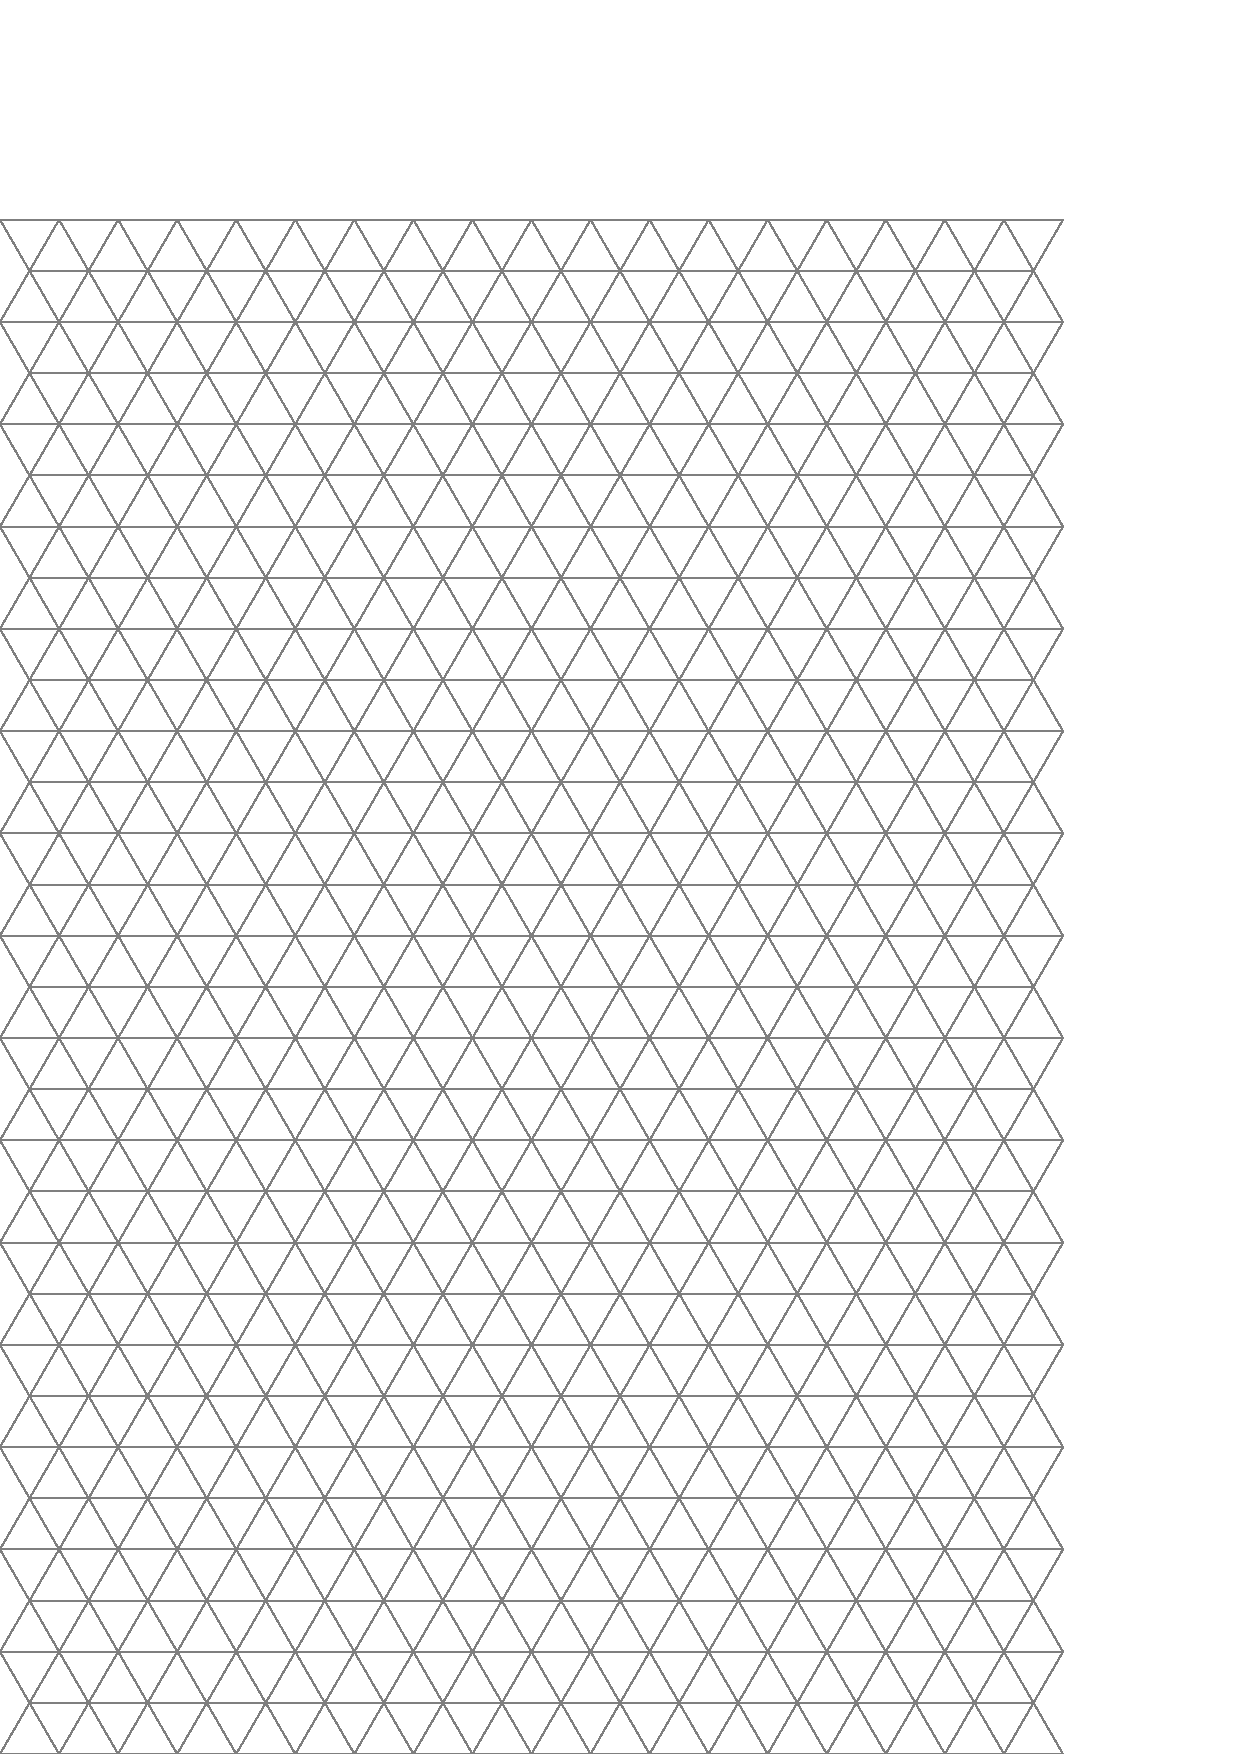
\includegraphics{triangle.0}
	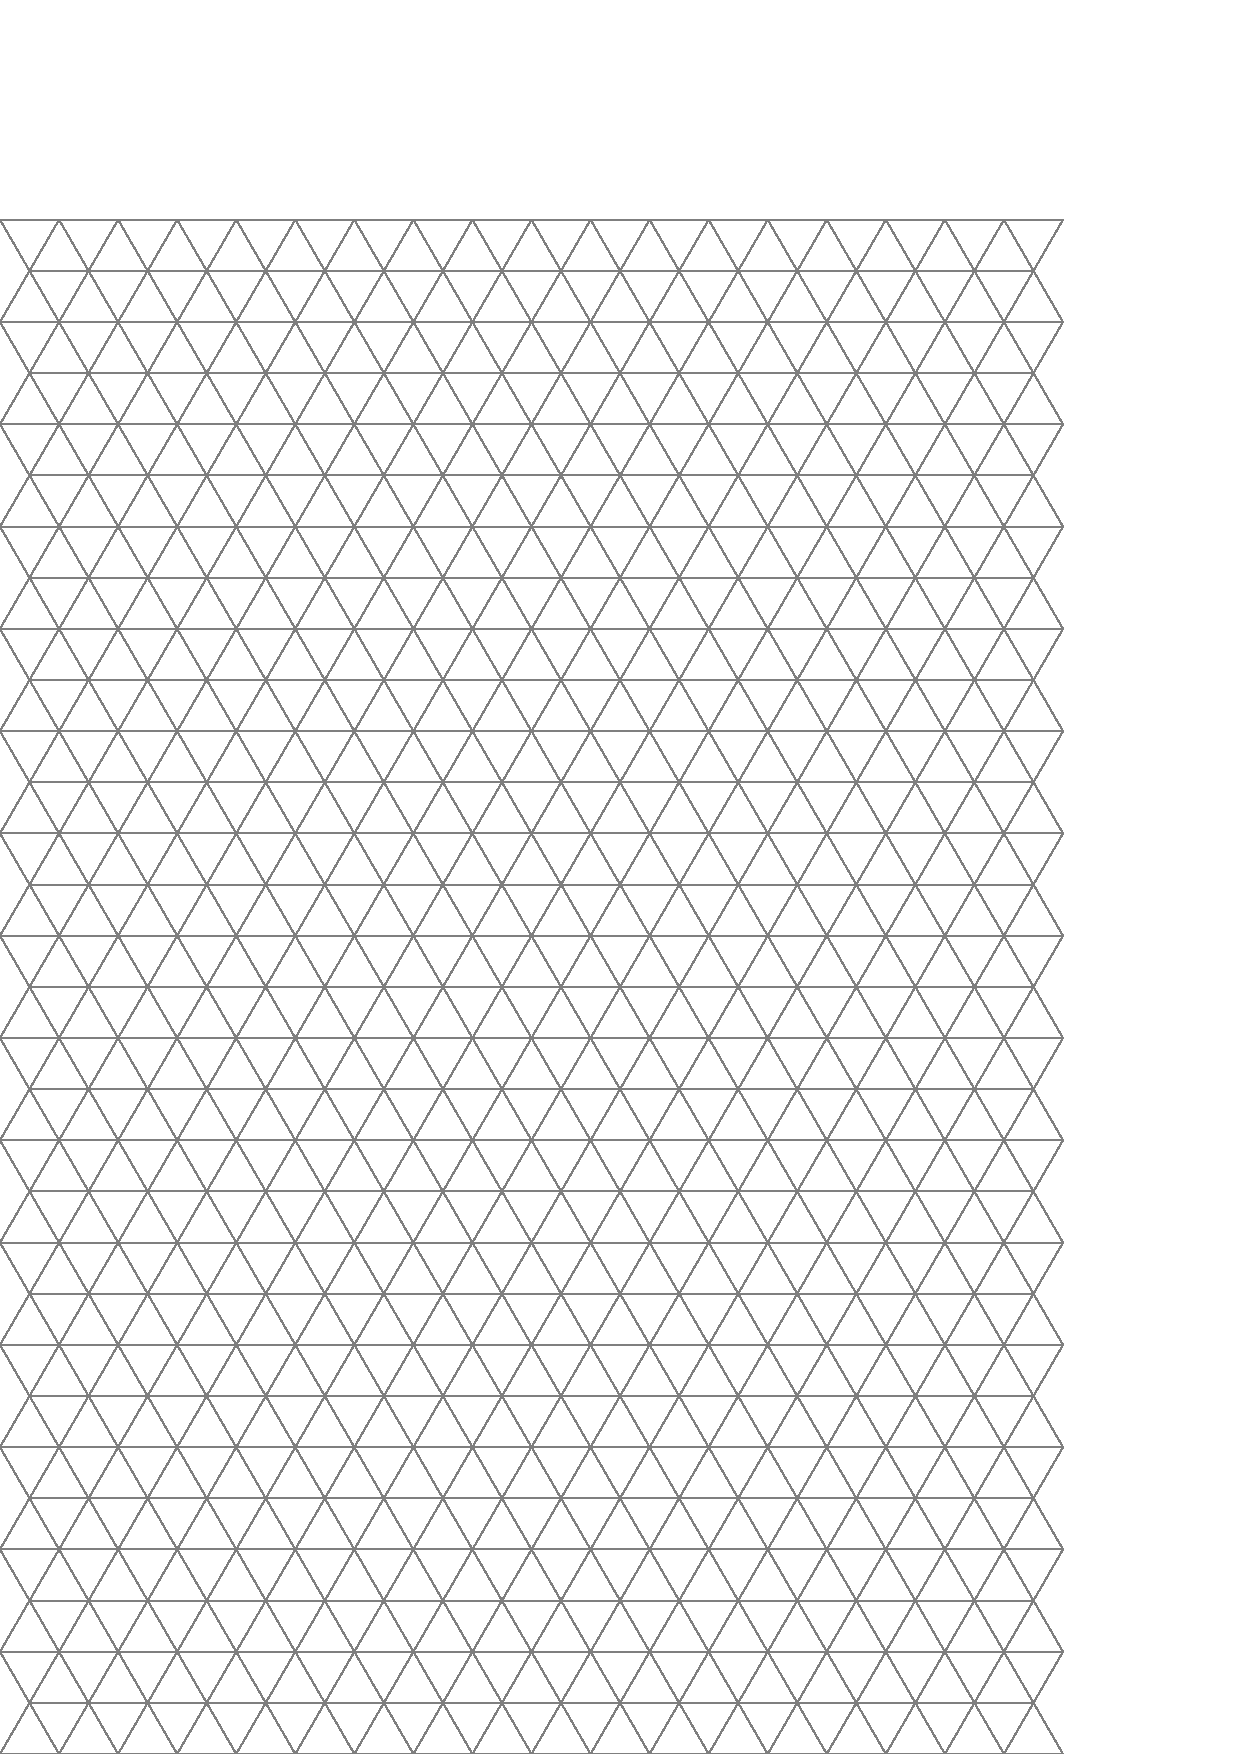
\includegraphics[scale=.98]{triangle.0}
%\end{center}

\label{LastPage}
\end{document}

